\documentclass[journal]{IEEEtran} % use the `journal` option for ITherm conference style
\IEEEoverridecommandlockouts
% The preceding line is only needed to identify funding in the first footnote. If that is unneeded, please comment it out.
\usepackage{cite}
\usepackage{amsmath,amssymb,amsfonts}
\usepackage{algorithmic}
\usepackage{graphicx}
\usepackage{textcomp}
\usepackage{xcolor}
\def\BibTeX{{\rm B\kern-.05em{\sc i\kern-.025em b}\kern-.08em
    T\kern-.1667em\lower.7ex\hbox{E}\kern-.125emX}}
\begin{document}

\title{Identificación de Clusters Temáticos en Correos Electrónicos\\
% delete or comment-out the following line before submission
{\footnotesize Práctica 3: Aplicación de Business Intelligence y Minería de Datos}
\thanks{Identify applicable funding agency here. If none, delete this.}
}

\author{%%%% author names
    \IEEEauthorblockN{ Gaston Humberto Nina Sossa}% first author
    % duplicate the line above as many times as needed to list all authors
    \\%%%% author affiliations
    \IEEEauthorblockA{\textit{Postgrado de Informatica, Universidad Mayor de San Andres}}\\% first affiliation
    % duplicate the line above as many times as needed to list all affiliations
    %%%% corresponding author contact details
    \IEEEauthorblockA{gastonnina@gmail.com}
}
\maketitle

\begin{abstract}
    Este documento describe un análisis de agrupamiento temático de correos electrónicos. Se hizo uso de varias técnicas de procesamiento de lenguaje natural, incluyendo limpieza de texto, tokenización, eliminación de stopwords y stemming. Los textos fueron vectorizados utilizando el método de TF-IDF y luego agrupados con el algoritmo K-Means. El número óptimo de clústeres se evaluó utilizando el método del codo y el índice de Silhouette, determinando que siete grupos proporcionaban un razonable equilibrio entre simplicidad y calidad de separación. Tambien se realizó el análisis de PCA y metadatos que demostraron que los clústeres generados reflejaban temas coherentes como hardware, software, religión, deportes y sociedad, lo cual fue una fuerte evidencia de la efectividad del enfoque no supervisado para segmentar contenido textual diverso.
\end{abstract}


\section{Introducción}
El análisis automático de grandes volúmenes de texto se ha convertido en una herramienta clave para extraer conocimiento en contextos donde no existe una estructura previa definida. En este trabajo se aborda el problema de descubrir temáticas latentes en un conjunto de correos electrónicos provenientes de foros públicos, los cuales abarcan una amplia gama de temas como tecnología, deportes, sociedad y religión. Dado que estos documentos no están etiquetados, se recurrió a técnicas de procesamiento de lenguaje natural (NLP) y aprendizaje no supervisado para identificar agrupaciones de contenido similares. El objetivo principal es evaluar si es posible organizar este grupo de correos de forma significativa, permitiendo así una mejor comprensión de los temas abordados por los usuarios en estos espacios de discusión.

\section{Objetivo}
El objetivo de este trabajo es aplicar técnicas de procesamiento de texto y algoritmos de agrupamiento no supervisado para identificar y analizar temáticas recurrentes en un conjunto de correos electrónicos. Se busca evaluar la capacidad del modelo para segmentar el conjunto de documentos de forma coherente, sin necesidad de etiquetas previas.

\section{Metodología}

La presente investigación se desarrolló bajo un enfoque cuantitativo y exploratorio, empleando técnicas de Procesamiento de Lenguaje Natural (NLP) y Minería de Datos para descubrir patrones temáticos en un conjunto de correos electrónicos públicos provenientes de foros de discusión. El objetivo fue identificar agrupaciones semánticas sin etiquetas previas, a partir de la similitud textual entre documentos.

El proceso metodológico se estructuró siguiendo las fases del ciclo de vida de un proyecto de análisis de texto:

\begin{itemize}
    \item Carga y exploración de los datos
    \item Preprocesamiento textual
    \item Representación vectorial del contenido
    \item Minería de datos mediante algoritmos de agrupamiento
    \item Visualización e interpretación de resultados
\end{itemize}

A continuación, se detallan los componentes clave aplicados en cada etapa del proceso.

\subsection{Preprocesamiento del texto}
Se aplicaron técnicas básicas de limpieza como la conversión a minúsculas, eliminación de signos de puntuación, tokenización, eliminación de palabras vacías (\textit{stopwords}) y stemming. Este último se realizó con Snowball Stemmer debido a su eficiencia frente a la lematización, especialmente en tareas de clustering donde no se requiere una precisión gramatical completa \cite{manning2008introduction}.

\subsection{Vectorización del contenido}
Para representar los textos como vectores numéricos, se utilizó el modelo TF-IDF (\textit{Term Frequency–Inverse Document Frequency}), que pondera los términos según su relevancia relativa en el conjunto. Esta técnica permite capturar las palabras distintivas de cada documento y es ampliamente utilizada en tareas de clasificación y agrupamiento \cite{ramos2003using}.

\subsection{Agrupamiento no supervisado}
El algoritmo K-Means fue utilizado para identificar patrones temáticos en los vectores TF-IDF. Este método busca minimizar la distancia intra-cluster y es eficiente para trabajar con grandes volúmenes de datos de alta dimensión \cite{lloyd1982least}.

\subsection{Determinación del número óptimo de clusters}
Para seleccionar un valor adecuado de $k$, se aplicaron dos métricas de validación interna: el método del codo, que observa la variación de la inercia, y el índice de Silhouette, que mide la coherencia interna de los grupos \cite{rousseeuw1987silhouettes}. Ambos indicadores sugirieron un rango entre 6 y 10, optando por $k=7$ por su buen equilibrio entre simplicidad y separación.

\subsection{Visualización de resultados}
Se utilizó Análisis de Componentes Principales (PCA) para reducir la dimensionalidad de los vectores TF-IDF a dos dimensiones. Esto permitió visualizar la distribución de los clusters y validar gráficamente la coherencia de las agrupaciones.

\section{Desarrollo}

A lo largo del proyecto se siguió una metodología estructurada, compuesta por seis etapas principales. Cada una de ellas se diseñó para garantizar la correcta transformación, análisis y visualización del contenido textual contenido en los correos electrónicos.

\subsection*{1. Carga y exploración del conjunto de datos}
Se cargaron archivos en formato \texttt{.txt}, cada uno correspondiente a un correo electrónico individual. En esta etapa se identificó el número total de documentos, la longitud promedio de los textos y se visualizaron ejemplos concretos de asuntos y cuerpos de mensajes. Esta exploración permitió verificar la diversidad temática y la necesidad de limpiar el texto antes de aplicar técnicas automáticas.

\vspace{12pt}
El conjunto de datos está compuesto por \textbf{18,728 correos electrónicos} en formato texto plano, cada uno representando un mensaje independiente proveniente de foros públicos. Durante la etapa inicial se realizó una exploración para entender la estructura y características generales del contenido.

\vspace{12pt}
Se extrajeron metadatos relevantes como el remitente, asunto del correo, si el mensaje era una respuesta (identificado por el prefijo \texttt{Re:}) y si contenía citas (líneas que inician con el símbolo \texttt{>}). Esta información permitió caracterizar el tipo de mensajes contenidos y establecer relaciones entre ellos, como se muestra en la Tabla~\ref{tab:estructura-dataset}.

\begin{table*}[t]
\centering
\caption{Ejemplo de estructura del dataset después del preprocesamiento}
\label{tab:estructura-dataset}
\resizebox{\textwidth}{!}{%
\begin{tabular}{|l|r|l|l|c|p{4.5cm}|c|c|}
\hline
\textbf{Archivo} & \textbf{Long.} & \textbf{From} & \textbf{Subject} & \textbf{Resp.} & \textbf{Body (inicio)} & \textbf{Cita} & \textbf{Nivel} \\
\hline
620ee9\ldots.txt & 2177 & ervan@rice.edu (Ervan Darnell) & Re: Limiting Govt\ldots & True & In article \textless{}1993Apr18.172531.10946@isc-br\ldots & False & 0 \\
a1c3fd\ldots.txt & 1828 & harvey@oasy\ldots & Re: Is MSG sensitivity\ldots & True & In rec.food.cooking, packer@delphi\ldots & True & 1 \\
51039c\ldots.txt & 1864 & jmd@cube.h\ldots & Re: ATF BURNS\ldots & True & In article \textless{}1993Apr20.143255.12711@mcs.kent.edu\ldots & True & 1 \\
08f918\ldots.txt & 6976 & MANDTBACKA@FINABO\ldots & After 2000 years\ldots & True & In \textless{}1r34n3$fhj@horus\ldots & True & 1 \\
c1f19f\ldots.txt & 1531 & rogue@ccs\ldots & Re: Clipper considered\ldots & True & In article \textless{}rcboi$j4a@access\ldots & True & 1 \\
\hline
\end{tabular}%
}
\end{table*}

\vspace{12pt}
Del total de correos, el 65.9\% (12,350) fueron identificados como respuestas, mientras que el 34.1\% correspondieron a mensajes originales. Además, el 50.19\% de los correos contienen al menos una cita textual, lo que refleja una alta frecuencia de mensajes en formato de conversación.

\vspace{12pt}
En la Figura~\ref{fig:niveles-cita}, se observa la distribución de niveles máximos de cita encontrados en los mensajes. La mayoría de los correos contienen entre 0 y 2 niveles de cita, aunque en algunos casos se alcanzan hasta 6 niveles, lo que indica mensajes con cadenas de respuestas anidadas.

\begin{figure}[H]
    \centering
    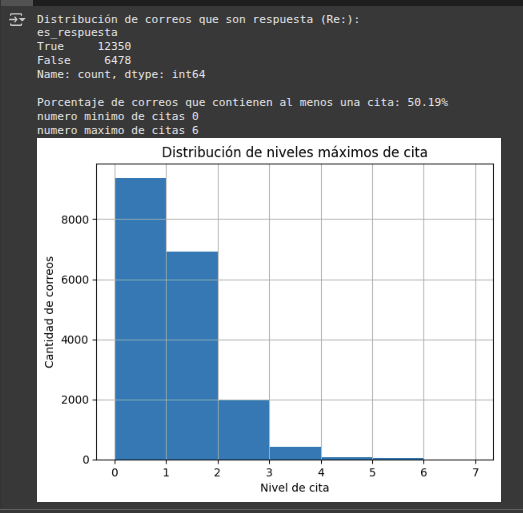
\includegraphics[width=0.7\linewidth]{fig1.png}
    \caption{Distribución de niveles máximos de cita en los correos electrónicos}
    \label{fig:niveles-cita}
\end{figure}

\subsection{2. Preprocesamiento del texto}
El preprocesamiento fue clave para eliminar elementos irrelevantes y homogenizar el contenido textual. Se aplicaron las siguientes transformaciones:
\begin{itemize}
    \item Conversión de texto a minúsculas
    \item Eliminación de puntuación y símbolos no alfabéticos
    \item Tokenización en palabras
    \item Eliminación de palabras vacías (\textit{stopwords})
    \item Aplicación de \textit{stemming} con Snowball Stemmer
\end{itemize}

Se eligió \textit{stemming} en lugar de lematización debido a su eficiencia computacional, considerando que el objetivo del proyecto no requería un análisis lingüístico profundo, sino una representación coherente para clustering.

\subsection{3. Vectorización del texto}
Para convertir los documentos en vectores numéricos, se utilizó el modelo TF-IDF (\textit{Term Frequency–Inverse Document Frequency}). Esta técnica pondera los términos según su frecuencia en el documento y su rareza en el conjunto global, permitiendo reducir el impacto de palabras comunes y resaltar aquellas más representativas. Se eligió TF-IDF por su simplicidad, rendimiento y efectividad demostrada en tareas de agrupamiento de texto.

\subsection{4. Análisis de clustering}
Se utilizó el algoritmo K-Means para agrupar los documentos en función de la similitud de sus vectores TF-IDF. Esta técnica fue seleccionada por su eficiencia con grandes volúmenes de datos y su adecuada compatibilidad con representaciones numéricas dispersas como las generadas por TF-IDF. K-Means permite identificar estructuras latentes en los datos sin supervisión ni etiquetas previas.

\subsection{5. Estimación del número óptimo de clusters}
Para determinar un valor adecuado de $k$, se evaluaron dos métricas:

\begin{itemize}
    \item El \textbf{método del codo}, que mide la disminución de la inercia (variación dentro del cluster).
    \item El \textbf{índice de Silhouette}, que evalúa la separación y coherencia de los grupos formados.
\end{itemize}

Ambas métricas sugirieron que valores entre 6 y 10 eran razonables. Se seleccionó $k=7$ por ofrecer un buen equilibrio entre simplicidad y separación efectiva, y porque los ejemplos explorados mostraban coherencia temática dentro de cada grupo.

\subsection{6. Visualización de resultados}
Para facilitar la interpretación de los clusters, se aplicó PCA (Análisis de Componentes Principales) con el fin de reducir la dimensionalidad de los datos TF-IDF a dos dimensiones. Esto permitió graficar los documentos en un plano 2D, donde fue posible observar visualmente la distribución de los grupos. Además, se generó un heatmap con variables como “es respuesta”, “tiene cita” y “nivel máximo de cita”, lo cual permitió caracterizar cada cluster en función del tipo de mensajes que lo componen.


\begin{thebibliography}{9}

\bibitem{manning2008introduction}
C. D. Manning, P. Raghavan, and H. Schütze, \textit{Introduction to Information Retrieval}. Cambridge University Press, 2008.

\bibitem{ramos2003using}
J. Ramos, “Using tf-idf to determine word relevance in document queries,” in \textit{Proceedings of the First Instructional Conference on Machine Learning}, 2003.

\bibitem{lloyd1982least}
S. P. Lloyd, “Least squares quantization in PCM,” \textit{IEEE Transactions on Information Theory}, vol. 28, no. 2, pp. 129–137, 1982.

\bibitem{rousseeuw1987silhouettes}
P. J. Rousseeuw, “Silhouettes: A graphical aid to the interpretation and validation of cluster analysis,” \textit{Journal of Computational and Applied Mathematics}, vol. 20, pp. 53–65, 1987.

\end{thebibliography}

\vspace{12pt}


\end{document}
